\documentclass[12pt]{article}
%Gummi|065|=)
\usepackage{graphicx}
\graphicspath{ {images/} }
\usepackage{titling}

\setlength{\droptitle}{-10em}   % This is your set screw
\title{\textbf{Sketch Recognition and Flow Chart Interpretation}}
\author{Alyssa Waln \\ 6.UAP Final Report \\ Supervisor: Randall Davis}
%\date
\begin{document}

\maketitle

\tableofcontents

\section{Introduction}
\par This project was centered around making a sketch recognition system that opened a dialogue between the system and the user. User sketches are run through a sketch recognition system made to recognize a small set of node shapes and edge types, converted to an internal representation, and returned to the user as a cleaner graph that can be moved around on the canvas. During this process, if the system wants to make a change it is unsure of, it will show the user a potential change and ask for clarification.\\

\par Originally, this project was made to streamline adding graphs to \LaTeX \ documents, as popular packages like TikZ\cite{TikZ} are powerful but not particularly intuitive. The internal representation could be quickly converted to \LaTeX \ code for insertion into documents. To focus on the representation portion of the project, the conversion aspect was removed, though code remains in the repository\cite{repo} for it to be re-implemented at a later time.

\par To be able to test the system on multiple touchscreen devices, it is implemented entirely in JavaScript, and contained in a single web page at \texttt{http://awaln.github.io/UAT/}.

\section{Design Philosophy}
\par One thing that is difficult to capture from sketches is user intent. While there are many good sketch recognition systems, understanding what purpose the user had in mind is a much more difficult problem. Additionally, many problems in graph theory are very difficult, and out of the scope of this project. However, an easy (though possibly less satisfying) solution to some of these problems is to just ask the user. Thus a system that could ask the right questions could perform well, despite not knowing exactly what to do.\\

\par The focus of this project was not on perfect sketch recognition through training. Instead, the system is entirely enclosed in a client side web page, and retains no knowledge of previous uses. This makes the system more accessible from different devices such as touchscreen tablets and phones. The system relies on being able to say how confident it is in a particular answer, and if that is below a threshold, it will ask the user for clarification. Additionally, the system will try to organize the nodes of the graph from top to bottom based on the longest path through the graph. Again, this is shown as a suggestion to the user, and the user may revert the graph to its original shape if they desire.

\section{Sketch Recognition}
% a walkthrough of calling recognize_all
Originally, sketch recognition occurred as soon as the user stopped writing. However, this was found to be unhelpful and replaced with a button that the user pushed when they were ready to have their drawing converted. This button now calls the old \texttt{recognize} function once per drawing stroke.\\

\par Each stroke consists of three sets of data: one list each for x and y position data, and one list of time data.

\subsection{Closed versus Open Shapes}

\par Determining if a shape is closed versus open is decided in \texttt{\\\textbackslash js\textbackslash sketch\_recognition.js} by the \texttt{recognize} function, based on the location of the start and end points of the stroke. The distance between these two points is calculated as a percentage of the total stroke length and that value is compared to a threshold. If it is above the threshold, the shape is considered open. If not, the shape is considered closed. This threshold was empirically determined to work well at 10\% of the total stroke length.\\

\par This detection allows a very important aspect of sketching: when a user traces the outline of a shape over and over, often to give it a more concrete shape, the shape can still be detected very accurately, since the distance between the start and endpoint as a percentage of stroke length only decreases with the number of retracings a user makes. Previous iterations of the design only checked the distance between the start and end points, without taking the total stroke length into account, and suffered in this aspect as a result.

\subsection{Corner Detection}
\par \texttt{recognize} calls a second function in the same file, \texttt{count\_corners}, which uses a similar method to that in \cite{project1} to estimate the number of corners in the given stroke. The two basic methods are to estimate local minima of speed under a speed threshold, and local maxima of curvature above a threshold that are also below a second speed threshold.\\

\par Determining speed is done by taking the stroke point by point, and estimating the speed between the two based on the location and time data. Curvature is more complex, first finding the slopes between points, and converting into arctangents. While doing this, the system must also recognize when the values of the arctangents ``flip'' from negative to postive at $\pm \pi/2$, and augment them so they continute smoothly in whatever direction they were initially going, as shown in Figure \ref{arctans}.\\

\begin{figure}
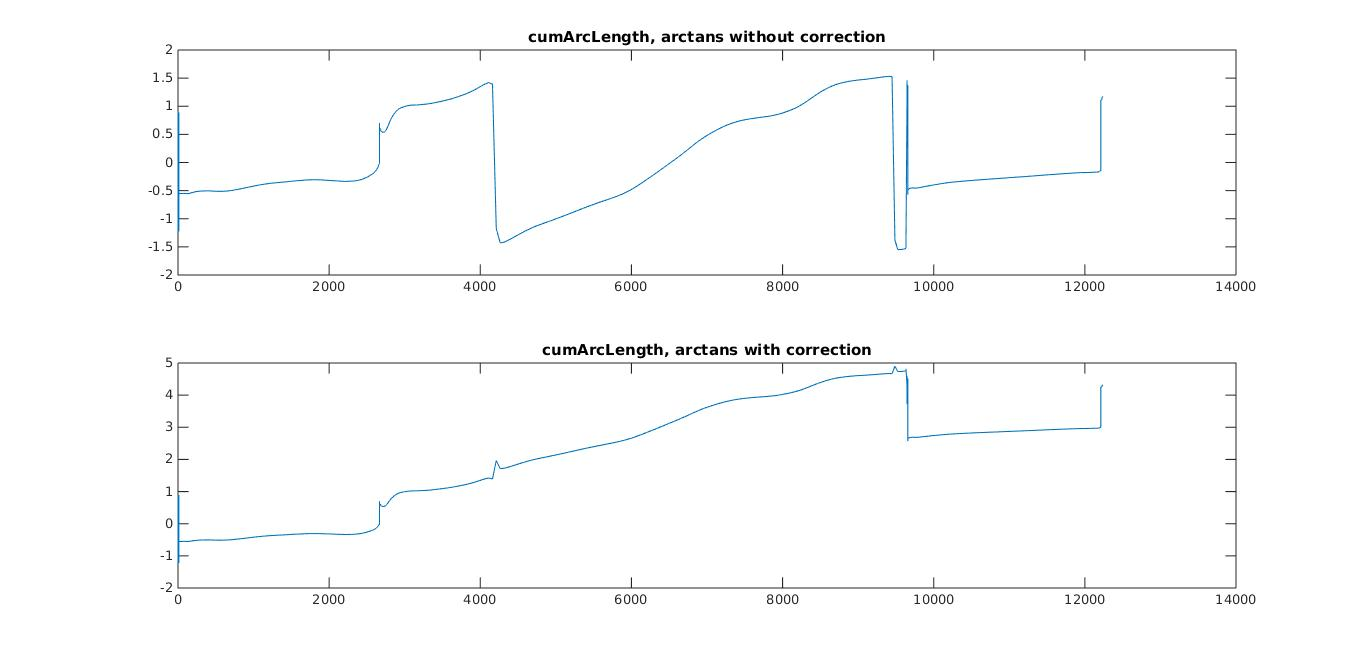
\includegraphics[width=\textwidth]{question4corrected.jpg}
\caption{An example of arctangent values before correction (above) and after correcting to make the function more continuous.}
\label{arctans}
\end{figure}

\par Once potential corners are located, they are passed back to \texttt{recognize} and used in determining the final shape of the node, if it is determined to be a polygon. The determination between a circle and a polygon is done by regression testing on the lines created by the found corners. If the line segments the corners create fit poorly to the points that exist between the corners, the sides of the potential polygon are considered too curved, and the shape is classified as a circle with some confidence. If they fit reasonably well, the shape is classified as a polygon with some confidence. Confidence levels are explained in the next subsection.\\

\par Corner detection is still used on open shapes (edges) and determined whether a line was meant as an undirected or directed edge, on the assumption that directed edges would be drawn with arrowheads. However, this distinction was no longer used after the \LaTeX conversion was cut, though the distinction does remain in the code.

\subsubsection{Confidence}
Indicating confidence levels for shape recognition was inspired by \cite{paleosketch}, though implementation differed greatly due to a lack of training sets. For circles, the confidence level is chosen as $$1 - (\textit{average coefficient of determination between corners})$$
For example, if the system detected three corners and the linear regression fit $R^2$ values were .6, .7, and .8, the confidence value for that shape being a circle would be $1 - (.6+.7+.8)/3 = .3$. Since those indicate a pretty good fit, the system is not confident the shape is a circle.\\

\par The confidence for polygons was set at .7, as this was found to be the circle confidence at which the system began to make frequent errors.

\section{Internal Representation}
% an explanation of the drawing object and why it is terrible.
Sketch components are saved in one large object called \texttt{drawing}, which consists of \texttt{nodes, edges, arrows, loners, edgelabels}, and \texttt{nodelabels}. \texttt{Edgelabels} and \texttt{nodelabels} are no longer used (part of the \LaTeX conversion) but remain in the code.
\subsection{Nodes}
\par \texttt{nodes} contains all nodes of the graph. Nodes are stored with confidence levels for circular or polygonal shape, a center x and y value, a ``radius,'' and a list of the corners that \texttt{count\_corners} found.\\
\par Since circular nodes were implemented first, much of the structure (i.e., having nodes represented by a point and a radius) was an easy way for the rest of the functions to access nodes. The center and radius are calculated by first averaging all the location values to get the center of all points, and then getting the average distance to the center as the radius. This fully describes circular nodes and helps estimate the footprint of polygons.
\subsection{Edges} % The fact that they are not stored by location is important!
\par Once a stroke is recognized as an open stroke, it is checked to see if the ends fall within a node. To be a bit more lenient with polygons, the radius is used to decide if a stroke starts or ends within any node, not just circular nodes. If it does, it is considered an edge and stored in \texttt{drawing.edges} as a start and end point only, where these points are the center of whatever nodes they are attatched to. Since this means edges are only defined by what they connect, it is much easier to move them when nodes are shifted in the graph.
\subsubsection{A Note About Arrows}
\par Though not used as arrows, if an open shape has corners it is saved in \texttt{drawing.arrows} instead of \texttt{drawing.edges}. Both are considered as edges for later computation.
\subsection{Unlinked Edges} % loners
\par If an open stroke has one or both ends \textit{not} fall within the radius of a node, it is considered a ``loner'' and drawn in red as a straight line from the start of the stroke to the end of the stroke. If a node is drawn later that covers the open endpoint(s), the loner is immediately converted to an edge between the nodes that now lie at its endpoints.

\section{Drawing Returned To User}
% an explanation of drawing on canvas
On hitting the ``convert'' button, the drawing that the user sketches is erased, replaced by an HTML canvas computer-drawn graph of the representation it determined from the user's sketch.
\subsection{Drawing Nodes and Edges}
\par Edges are drawn first as straight lines from the center of the start nod to the center of the end node. Nodes are drawn over this and filled in white to make the edges seem to stop around the edge of the node. Circular nodes are drawn as full arcs at their radius away from their center point. Polygonal nodes are drawn as line segments from one corner to the next.
\subsection{Moving Nodes}
\par When in ``Move Mode,'' the user can click and drag nodes on the canvas. Every time the user moves, a re-draw of the canvas is triggered. As mentioned before, since the edges are defined by their end nodes, edges automatically move with nodes.\\
\par Regardless of node shape, all nodes are shifted over by noting the vector the mouse has travelled, and adding it to the center of the node, as well as all corners.\\
\par Finding out whether the user has clicked within a polygon was actually the most difficult part of this process, as the polygons could be concave. The system decides if a point is within a polygon by determining if a ray starting from that point and heading directly right intersects an odd number of edges, based on the approach in \cite{doIntersect}.

\section{Sketch Interpretation}
% a walkthrough of all the ask functions
Using the confidence values and edge list calculated earlier, the system will ask about any nodes it is not very certain of and about potential reorganizations. The following functions, unless specified, are all in \texttt{\textbackslash js\textbackslash canvas.js}.
\subsection{Node Shape}
\par The first time a node is recognized, it is marked as being not ``known.'' The system draws it as the shape it thinks most likely, then asks if this is the correct interpretation, shown in Figure \ref{ask_user1}.

\begin{figure}
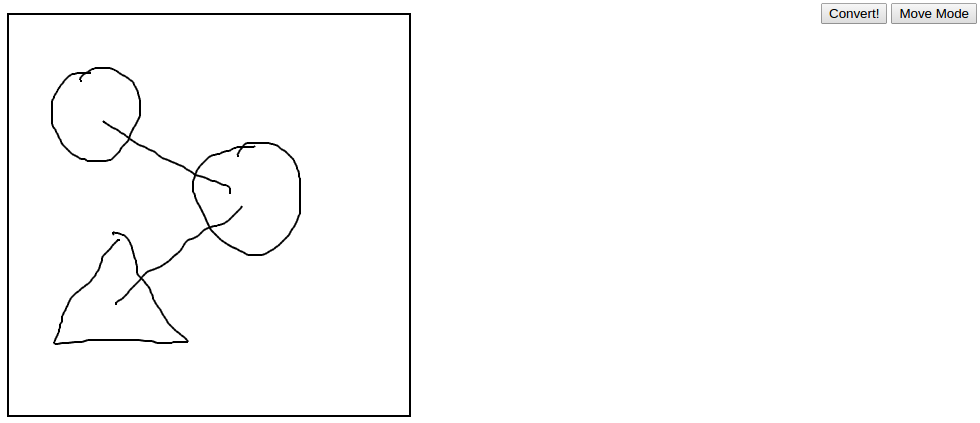
\includegraphics[width=\textwidth]{sketch.png}
\caption{The user-drawn sketch, before recognition.}
\label{sketch}
\end{figure}

\begin{figure}
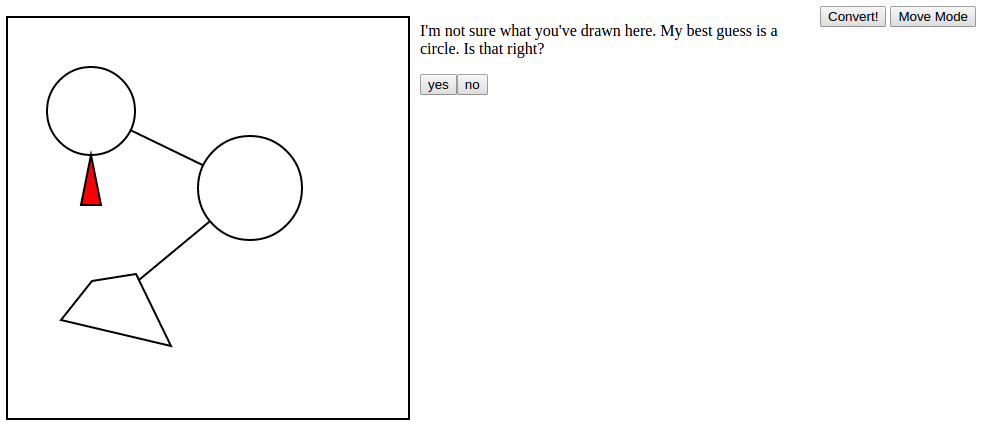
\includegraphics[width=\textwidth]{ask_user1.png}
\caption{After recognition, \texttt{ask\_user\_nodes} runs and asks the user if it picked the right shape.}
\label{ask_user1}
\end{figure}

\subsubsection{Callback}
\par Clicking ``yes'' or ``no'' triggers a callback function that marks the node's shape as ``known'' and updates the shape confidences to reflect this. It will also call \texttt{ask\_user\_nodes} again, which will bring up the dialogue again for the next node, shown in Figure \ref{ask_user3}. This cycle continues until there are no more nodes to evaulate, and \texttt{ask\_user\_nodes} will terminate with a value of 0, which indicates to the system to begin calling \texttt{ask\_user\_organize}.

\begin{figure}
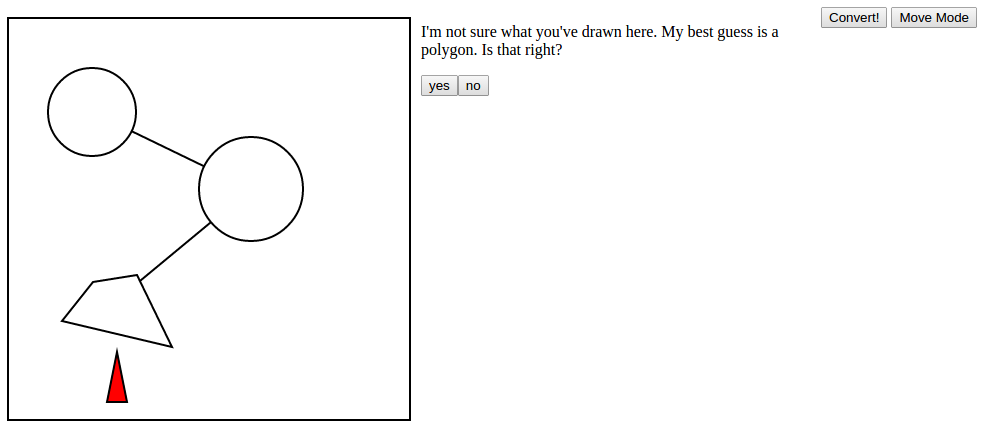
\includegraphics[width=\textwidth]{ask_user3.png}
\caption{On callback, if there are still nodes to evaluate, \texttt{ask\_user\_nodes} runs and asks the user if it picked the right shape.}
\label{ask_user3}
\end{figure}

\subsection{Node Organization}
\par \texttt{ask\_user\_organize} will try to reorganize the graph from top to bottom in a straight line along the longest path through the graph, if possible. It calls \texttt{longest\_path} for the longest path computation in \texttt{\textbackslash js\textbackslash sketch\_recognition.js}.\\

\par The longest path in a graph is known to be an NP-hard problem, and not known to be solvable in polynomial time. If the graph had a thousand nodes, this would be a serious issue as computation time would increase exponentially with the number of nodes. However, in the context of this graph interpretation, it is safe to assume a user will not want or be able to draw anywhere near one thousand nodes, so an exponential runtime for finding the longest path is acceptable.\\

\par The function \texttt{longest\_path} runs a British Museum algorithm, checking every possible start node and expanding outward in every possible direction until it reaches a node already in the path, and returning the longest path it finds from any start node, ordered to make the first node higher on the current graph than the last node (if this is not true, it will reverse the path before returning it).\\

\par Now with the longest path information \texttt{ask\_user\_organize} will save the orignal positioning and edit the drawing to align all the nodes in the path along the vertical axis if they will fit. Another set of buttons will appear asking the user if they wish to keep the changes, shown in Figure \ref{reorder} (a reordering of Figure \ref{ask_user3}).

\begin{figure}
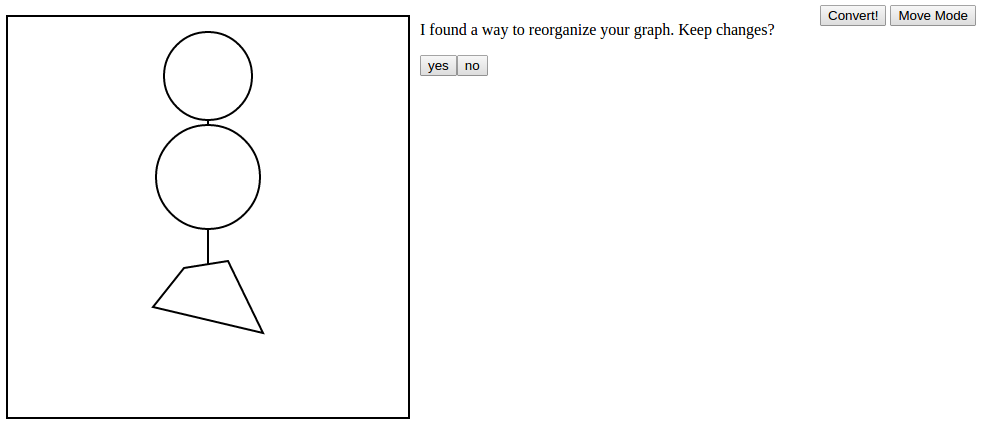
\includegraphics[width=\textwidth]{reorder.png}
\caption{A reordering of Figure \ref{ask_user3} suggested by the system.}
\label{reorder}
\end{figure}

\subsubsection{Callback}
\par Clicking ``yes'' or ``no'' triggers a callback function that will either keep the current drawing with the moved nodes, or replace the current drawing with the old copy of the drawing that was saved before the repositioning.

\section{Conclusion}
\par Though unable to retain knowledge from one session to the next, this system is able to ask simple questions to be more certain of user intent. Basic shapes are recognizable at a high level of granularity, and the question-and-answer interface could be extended to include more shapes easily. Future extensions of this project could use this style of interaction to further integrate the capabilities of human sketching and computer generated diagrams.\\

\par Additionally, I was unable to explore additional modalities in this project. Adding voice recognition could make interaction with the system more natural for users, mimicking a person dictating a graph to another person, except the latter person can draw perfect circles.

\begin{thebibliography}{5}
\bibitem{TikZ} 
TikZ and PGF home page
\\\texttt{http://www.texample.net/tikz/}
\bibitem{repo} 
Project Github Repository
\\\texttt{https://github.com/awaln/UAT}
\bibitem{project1} 
Stahovich, Thomas F. Segmentation of Pen Strokes Using Pen Speeds. \textit{Computers and Graphics, Volume 35, Issue 2, 2011,} pp. 250-264.
\bibitem{paleosketch} 
Paulson, Brandon, and Hammond, Tracy. Paleosketch: accurate primitive sketch
recognition and beautification. In \textit{Proceedings of IUI 08, ACM (New
York, NY, USA, 2008),} 1–10.
\bibitem{doIntersect}
Geeks for Geeks: How to check if two given line segments intersect?
\texttt{http://www.geeksforgeeks.org/check-if-two-given-line-segments-intersect/}
\end{thebibliography}


\end{document}
